\documentclass[14pt]{extarticle}

\usepackage[T2A]{fontenc}
\usepackage[utf8]{inputenc}
\usepackage[english,ukrainian]{babel}
\usepackage{bookmark}

\usepackage{amsmath,amssymb}
\usepackage{parskip}
\usepackage{graphicx}
\usepackage[table]{xcolor}
\usepackage{tcolorbox}
\tcbuselibrary{skins}
\usepackage[framemethod=tikz]{mdframed}
\usepackage{chngcntr}
\usepackage{enumitem}
\usepackage{hyperref}
\usepackage{float}
\usepackage{subfig}
\usepackage{chngcntr}
\usepackage{esint}
\usepackage{pdfpages} % Add this to your preamble

\usepackage{libertinus}

\usepackage[top=2.5cm, left=3cm, right=3cm, bottom=4.0cm]{geometry}
\usepackage{algorithm}
\usepackage{algpseudocode}
\usepackage{listings}
\usepackage{xcolor}

\definecolor{codegreen}{rgb}{0,0.6,0}
\definecolor{codegray}{rgb}{0.5,0.5,0.5}
\definecolor{codepurple}{rgb}{0.58,0,0.82}
\definecolor{backcolour}{rgb}{0.95,0.95,0.92}

\lstdefinestyle{mystyle}{
    backgroundcolor=\color{backcolour},   
    commentstyle=\color{codegreen},
    keywordstyle=\color{magenta},
    numberstyle=\tiny\color{codegray},
    stringstyle=\color{codepurple},
    basicstyle=\ttfamily\footnotesize,
    breakatwhitespace=false,         
    breaklines=true,                 
    captionpos=b,                    
    keepspaces=true,                 
    numbers=left,                    
    numbersep=5pt,                  
    showspaces=false,                
    showstringspaces=false,
    showtabs=false,                  
    tabsize=2
}
\lstset{style=mystyle}

\usepackage{ragged2e}
\begin{document}

\begin{titlepage}
	\centering
	%
\includegraphics[width=0.15\textwidth]{images/lab_1/logo.png}\par\vspace{0.3cm}
	{\textbf{Міністерство освіти і науки України}\par
 Харківський національний університет імені В.Н. Каразіна\par}
    \vspace{1cm}
	{\Large \textsc{Розрахунково-графічне завдання \#2}\par
    \textbf{Чисельне розв'язання крайових задач для звичайних диференціальних рівнянь}\par}
	\vfill
 \begin{FlushRight}
	\textbf{Виконав:}\par Захаров Дмитро Олегович \par Група МП-41
\end{FlushRight}
	\vfill

% Bottom of the page
	{\large Харків -- 2025\par}
\end{titlepage}

\tableofcontents
\pagebreak

\section{Постановка задачі}

Знайти розв'язок диференціального рівняння другого порядку 
з заданими граничними умовами:
\begin{equation*}
    y'' + x^3y' - (2+\ln^2(1+x))y = 3, \quad x \in (0,2)
\end{equation*}

Граничні умови:
\begin{equation*}
    -y'(0) + 3y(0) = 1, \quad y(2) = 2.
\end{equation*}

Розв'язок слід знайти з точністю $\varepsilon = 10^{-3}$ та 
побудувати графік розв'язку. Знайти розв'язок потрібно 
за допомогою хоча б одного з проекційних методів (метод Гальоркіна,
метод скінченних елементів, метод колокацій, метод найменших квадратів).

\pagebreak
\section{Опис методів}

Нехай маємо рівняння другого порядку
\begin{equation*}
    \begin{cases}
        \mathcal{L}[y] = y'' + p(x)y' + q(x)y = f(x), \quad x \in (a,b), \\
        e_0[y] := r_0y(a) + m_0y'(a) = \nu_0, \\
        e_1[y] := r_1y(b) + m_1y'(b) = \nu_1,
    \end{cases}
\end{equation*}

Будемо шукати розв'язок у вигляді
\begin{equation*}
    \widehat{f}(x|\boldsymbol{c}) = \varphi_0(x) + \sum_{i=1}^n c_i\varphi_i(x),
\end{equation*}

де $\{\varphi_j\}_{j \in \{0,\dots,n\}}$ --- лінійно незалежні базисні 
функції, причому $\varphi_0(x)$ має задовільняти початковим умовам, а решта 
функції задовільняють однорідним граничним умовам:
\begin{equation*}
    e_0[\varphi_0] = \nu_0, \quad e_1[\varphi_0] = \nu_1, \quad e_0[\varphi_j] = e_1[\varphi_j] = 0, \quad j \in \{1,\dots,n\}.
\end{equation*}

Наша задача --- підібрати так набір коефіцієнтів $\boldsymbol{c} = (c_0,\dots,c_n) \in \mathbb{R}^{n+1}$,
щоб зробити нев'язку $R(x|\boldsymbol{c})$ якомога меншою:
\begin{equation*}
    \textcolor{blue}{R(x|\boldsymbol{c}) = \mathcal{L}[\widehat{f}(x|\boldsymbol{c})] - f(x) = \mathcal{L}[\varphi_0(x)] + \sum_{i=1}^n c_i\left(\mathcal{L}[\varphi_i](x) - f(x)\right).}
\end{equation*}

Далі, кожен з методів по суті задає критерій ``малості'' нев'язки $R(x|\boldsymbol{c})$. 
Розглянемо два з них, що будемо використовувати в нашій роботі.

\subsection{Метод Гальоркіна}

Головна ідея в тому, що якщо б ми могли гарантувати, що нев'язка $R(x)$ є
ортогональною до всіх базисних функцій $\{\varphi_j(x)\}_{j \in \{0,\dots,n\}}$,
то тоді звідси б випливало, що $R \equiv 0$. Якщо б в нас був би нескінченний 
набір базисних функцій, то ми б могли задовольнити цю умову точно. В нашому 
ж випадку, ми підбираємо так коефіцієнти, щоб це виконувалось для 
перших $n$ базисних функцій:
\begin{equation*}
    \langle R(x|\boldsymbol{c}), \varphi_i(x) \rangle = \int_a^b R(x|\boldsymbol{c})\varphi_i(x)dx = 0, \quad i \in \{1,\dots,n\}.
\end{equation*}

Якщо розписати, то це зводиться до системи лінійних рівнянь:
\begin{equation*}
    \textcolor{green!50!black}{\sum_{j=1}^n \alpha_{i,j}c_j = \beta_{i}, \quad \alpha_{i,j} = \int_a^b \varphi_i(x)\mathcal{L}[\varphi_j]dx, \quad \beta_i = \int_a^b \varphi_i(x)(f(x)-\mathcal{L}[\varphi_0])dx.}
\end{equation*}

\subsection{Метод найменших квадратів}

Тут ми кажемо, що нев'язка $R(x|\boldsymbol{c})$ є малим числом в середньому, тобто
$\int_a^b R^2(x|\boldsymbol{c})dx$ є достатньо малим. Формально:
\begin{equation*}
    \mathcal{I}(\boldsymbol{c}) = \int_a^b R^2(x|\boldsymbol{c})dx \to \min
\end{equation*}

Ця задача оптимізації розв'язується стандартно: беремо градієнт
$\nabla_{\boldsymbol{c}} \mathcal{I}(\boldsymbol{c})$ і прирівнюємо до нуля:
\begin{equation*}
    \nabla_{\boldsymbol{c}} \mathcal{I}(\boldsymbol{c}) = 2\int_a^b R(x|\boldsymbol{c})\nabla_{\boldsymbol{c}}R(x|\boldsymbol{c})dx = \boldsymbol{0}_n \implies \textcolor{green!50!black}{\int_a^b R(x|\boldsymbol{c})\frac{\partial R(x|\boldsymbol{c})}{\partial c_i}dx = 0.}
\end{equation*}

\newpage

\section{Імплементація}
\label{sec:attached-pdf}

\subsection{Підбір параметрів}

В нашому випадку маємо підставити наступні значення та функції:
\begin{equation*}
    \mathcal{L}[y] = y'' + x^3y' - (2+\ln^2(1+x))y, \quad f(x) \equiv 3, \quad a=0, \quad b=2,
\end{equation*} 

Далі потрібно обрати базисні функції $\varphi_i(x)$, які задовольняють
граничним умовам:
\begin{gather*}
    -\varphi_0'(0) + 3\varphi_0(0) = 1, \quad \varphi_0(2) = 2, \\
    -\varphi_i'(0) + 3\varphi_i(0) = \varphi_i(2) = 0, \quad i \in \{1,\dots,n\}.
\end{gather*}

Функцією $\varphi_0(x)$ можна шукати як лінійну: $\varphi_0(x) = ax+b$. 
Нескладно перевірити, що підійде $\varphi_0(x) = \frac{5}{7}x + \frac{4}{7}$.

З функціями $\varphi_n(x), n \geq 1$ все складніше. Зокрема, з теорії 
диференціальних рівнянь, для такої умови можна взяти наступний 
ортогональний набір функцій:
\begin{equation*}
    \varphi_n(x) = \cos(\omega_n x) + \frac{3}{\omega_n}\sin(\omega_n x), \quad \tan (2\omega_n) = -\frac{\omega_n}{3}
\end{equation*}

Проте працювати з такими функціями не дуже зручно, тому спробуємо прибрати 
умову на ортогональність і візьмемо поліноміальний набір функцій:
\begin{equation*}
    \varphi_n(x) = (x-2)^n(a_nx+b_n)
\end{equation*}

Умова $\varphi_n(2) = 0$ виконується автоматично, лише підберемо 
коефіцієнти $a_n$ та $b_n$. Маємо отримати $-\varphi_n'(0) + 3\varphi_n(0) = 0$ або:
\begin{equation*}
    \left[-n(x-2)^{n-1}(a_nx+b_n) - a_n(x-2)^n + 3(x-2)^n(a_nx+b_n)\right]_{x=0} = 0
\end{equation*} 

Це спрощується до умови $-nb_n + 2a_n - 6b_n = 0$, звідки $a_n =
\frac{n+6}{2}b_n$. Візьмемо $b_n := 2$ для зручності. Тоді:
\begin{equation*}
    \varphi_0(x) = \frac{5}{7}x + \frac{4}{7}, \quad \varphi_n(x) = (x-2)^n\left(\left(6+n\right)x+2\right)
\end{equation*}

\subsection{Код на Wolfram Mathematica}

Код програми наведений на мові \textit{Wolfram Mathematica} у файлі, 
що прикріплений далі. 

\begin{center}
    \textbf{Перегорніть на наступну сторінку $\to$}
\end{center}

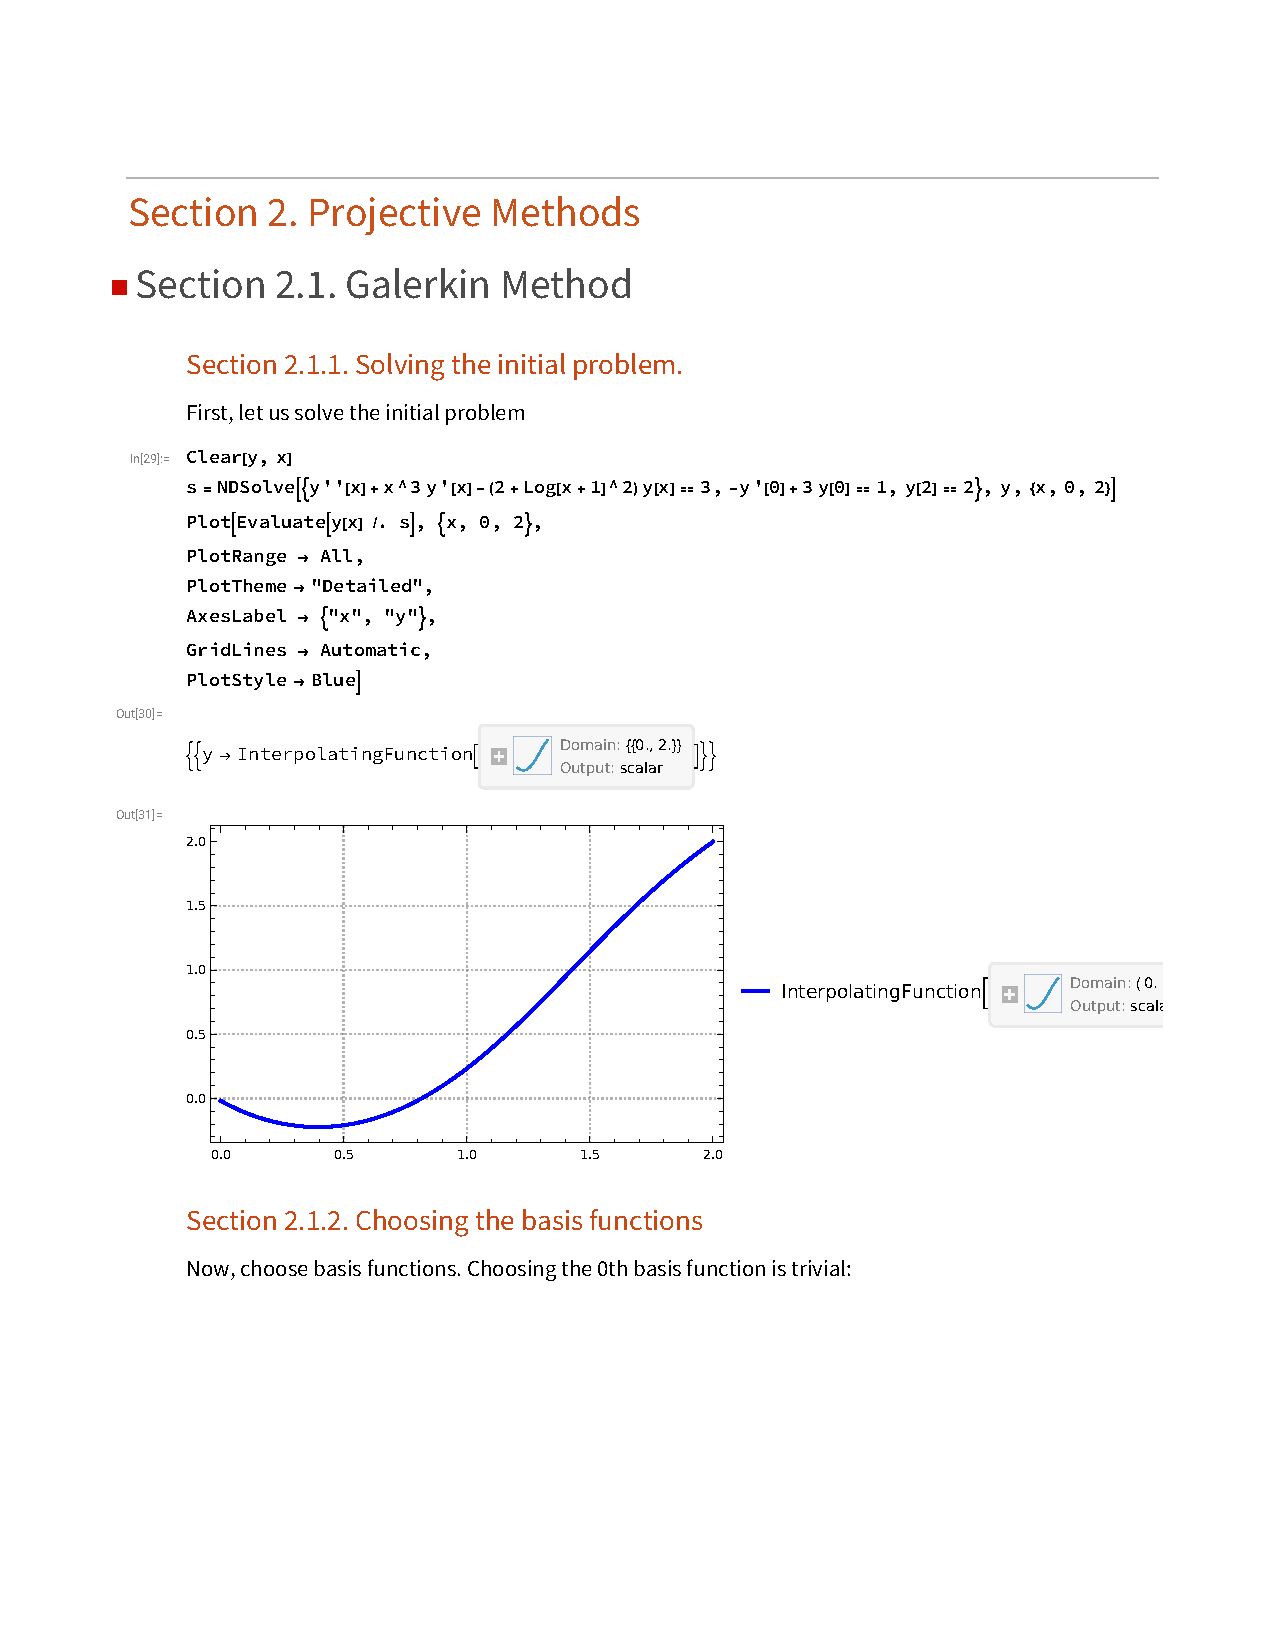
\includepdf[pages=-]{appendices/lecture-2-appendix.pdf}  % `pages=-` includes all pages

\end{document}

